\section{Results}

After building the circuit shown in Figure~\ref{f:astable} with the elements
listed in Table~\ref{t:elements}, the duty cycle and frequency of the output
were measured.  Figure~\ref{f:scope} shows an oscilloscope screenshot of such
measurements, and Table~\ref{t:error} aggregates the error in each
measurement.
%
\begin{figure}[H]
\centering
	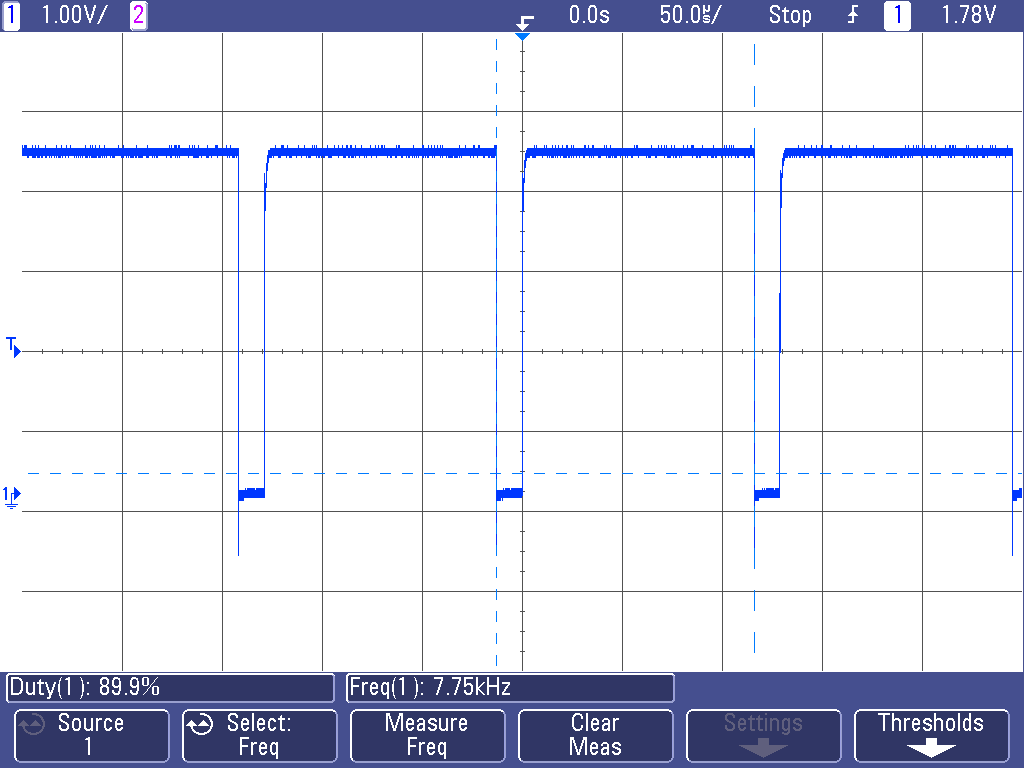
\includegraphics[width=.8\textwidth]{img/shot/555_output.png}
	\parbox{.8\textwidth}{
	\caption[Measured Results]{Oscilloscope screenshot of the constructed
	555-based timer's output.  Note the accuracy of the constructed system
	compared to the target~\SI{90}{\percent} duty cycle and~\SI{8}{\kilo\hertz}
	frequency.}
	\label{f:scope}}
\end{figure}
%
The system produced a nearly square wave with a frequency
of~\SI{7.75}{\kilo\hertz}, an error of just~\SI{-3.12}{\percent}.  Remarkably,
the observed duty cycle of the output exhibited an error of
just~\SI{-0.11}{\percent}, measuring~\SI{89.9}{\percent} compared to the
target~\SI{90}{\percent}.
%
\begin{table}[H]
\centering
	\parbox{.5\textwidth}{
	\caption[Measured Error]{Comparison of target and measured design
	parameters and their respective errors.}
	\label{t:error}}\\
	\begin{tabular}{|c|c|c|}
	\cline{2-3}
	\multicolumn{1}{c|}{} & \tbf{Duty Cycle} & \tbf{Frequency} \\ \hline
	\tbf{Target} & \SI{90}{\percent} & \SI{8}{\kilo\hertz} \\ \hline
	\tbf{Measured} & \SI{89.9}{\percent} & \SI{7.75}{\kilo\hertz} \\ \hline
	\tbf{Error} & \SI{-0.11}{\percent} & \SI{-3.12}{\percent} \\ \hline
\end{tabular}

\end{table}
